% ===========================================================================
%
%		FEDERICO II THESIS TEMPLATE - ENGLISH
%  					* an example of Chapter 2: mathematical text
%	 
% 		AUTHOR:  		Antonio Esposito (antonio.esposito103@studenti.unina.it)
%		LAST UPDATED:	2017/06/20
%
% ===========================================================================

\chapter{Desgin}
\section{Descrizione del dominio}
In seguito ad un'analisi dei requisiti del sistema si è resa evidente l'esistenza di alcune entità
principali:
\begin{itemize}
    \item gli \textit{Utenti} che possono registrarsi, visualizzare delle \textit{Strutture}
    e scrivere delle recensioni
    \item degli \textit{Amministratori} i quali possono gestire i dati dei visitatori e le loro recensioni
\end{itemize}
%%%%% ===============================================================================
\section{Analisi dell'architettura}
Il sistema si basa principalmente su due pattern architetturali: Client-Server e Model-View-Controller.\\
Il sistema infatti è composto da diversi client che tramite internet interagiscono con un Server remoto.
\begin{center}
    \begin{figure}[H]
        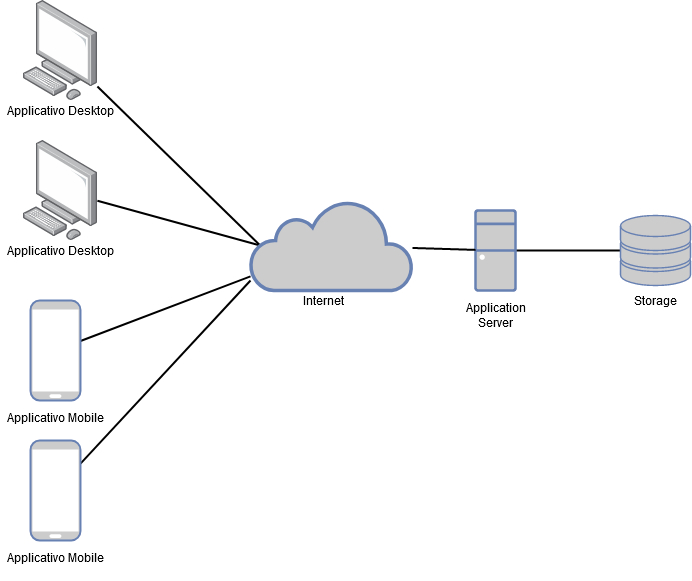
\includegraphics[width=\textwidth]{Figures/Architettura client server.png}
        \caption{Architettura client server}
    \end{figure}
\end{center}
\subsection{Model-View-Presenter}
Per quanto riguarda l'architettura interna dei client si è deciso di utilizzare il modello Model-View-Presenter (variante Passive View)
favorendo la separazione dei componenti software del sistema e separandone le responsabilità.
In questo modo si riesce ad ottenere alta coesione e basso accoppiamento, ottenendo una buona manutenibilà.\\
A favore di ciò il progetto è diviso in tre sottocartelle principali: Model, View e Presenter.\\
\\
Il modello MVP è un'evoluzione del modello Model View Controller ed è usato principalmente per creare user interfaces 
ed in particolare nella variante Passive View:
la componente \textbf{View} è completamente passiva e statica deputata soltanto alla visualizzazione dei dati.\\
la componente \textbf{Model} ha la responsabilità di fornire i metodi per accedere
ai dati utili all'applicazione, ha conoscenza del dominio applicativo ed è indipendente
dagli altri sottosistemi.\\
la componente \textbf{Presenter} fa da "middle man" tra la View ed il Model e si occupa di prendere i dati dal model, 
fornirli alla view e gestire gli input dell'utente
\begin{center}
    \begin{figure}[H]
        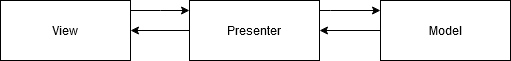
\includegraphics[width=\textwidth]{Figures/MVP client.png}
        \caption{Architettura Model-View-Controller}
    \end{figure}
\end{center}
\section{Diagramma delle classi di design}
\subsection{Applicativo Desktop}
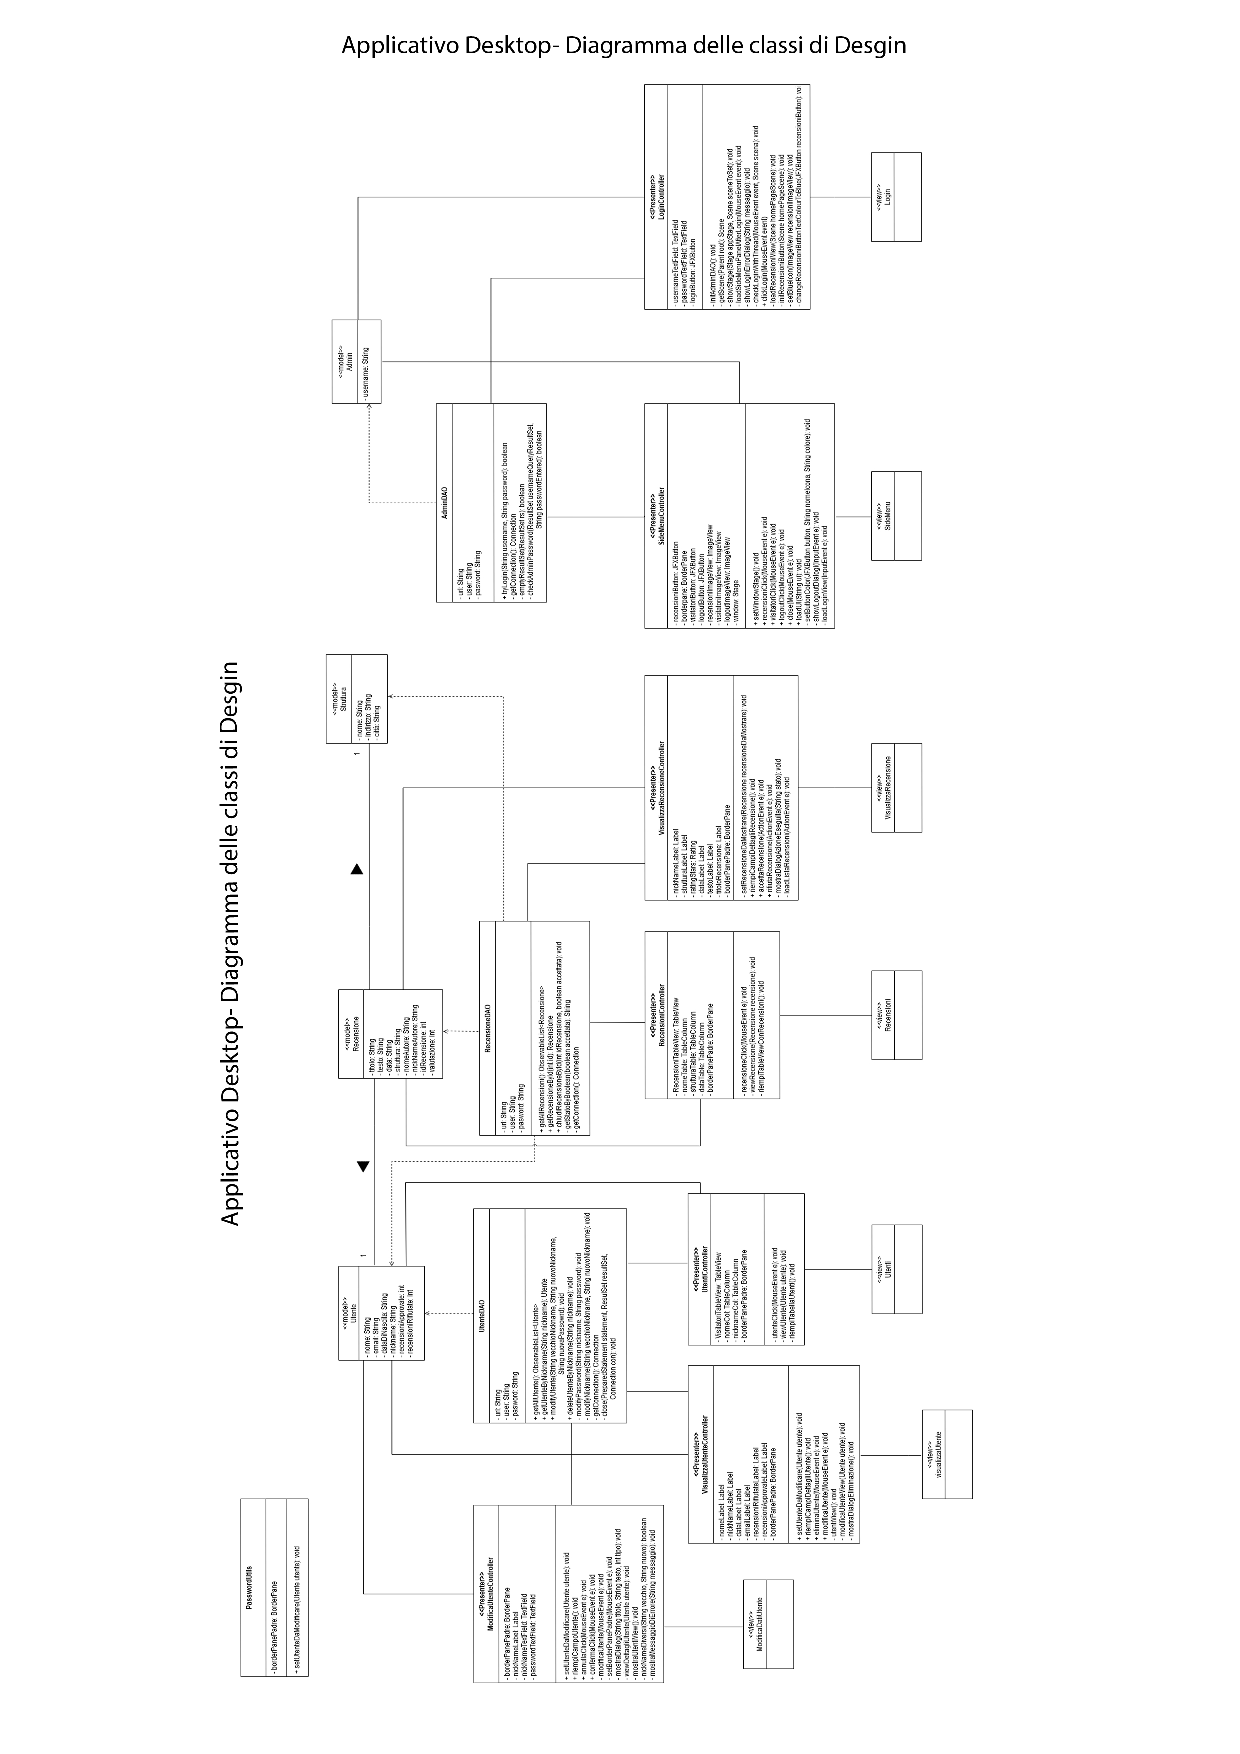
\includepdf{12.pdf}
%\begin{figure}[h!]
%   \centering
%    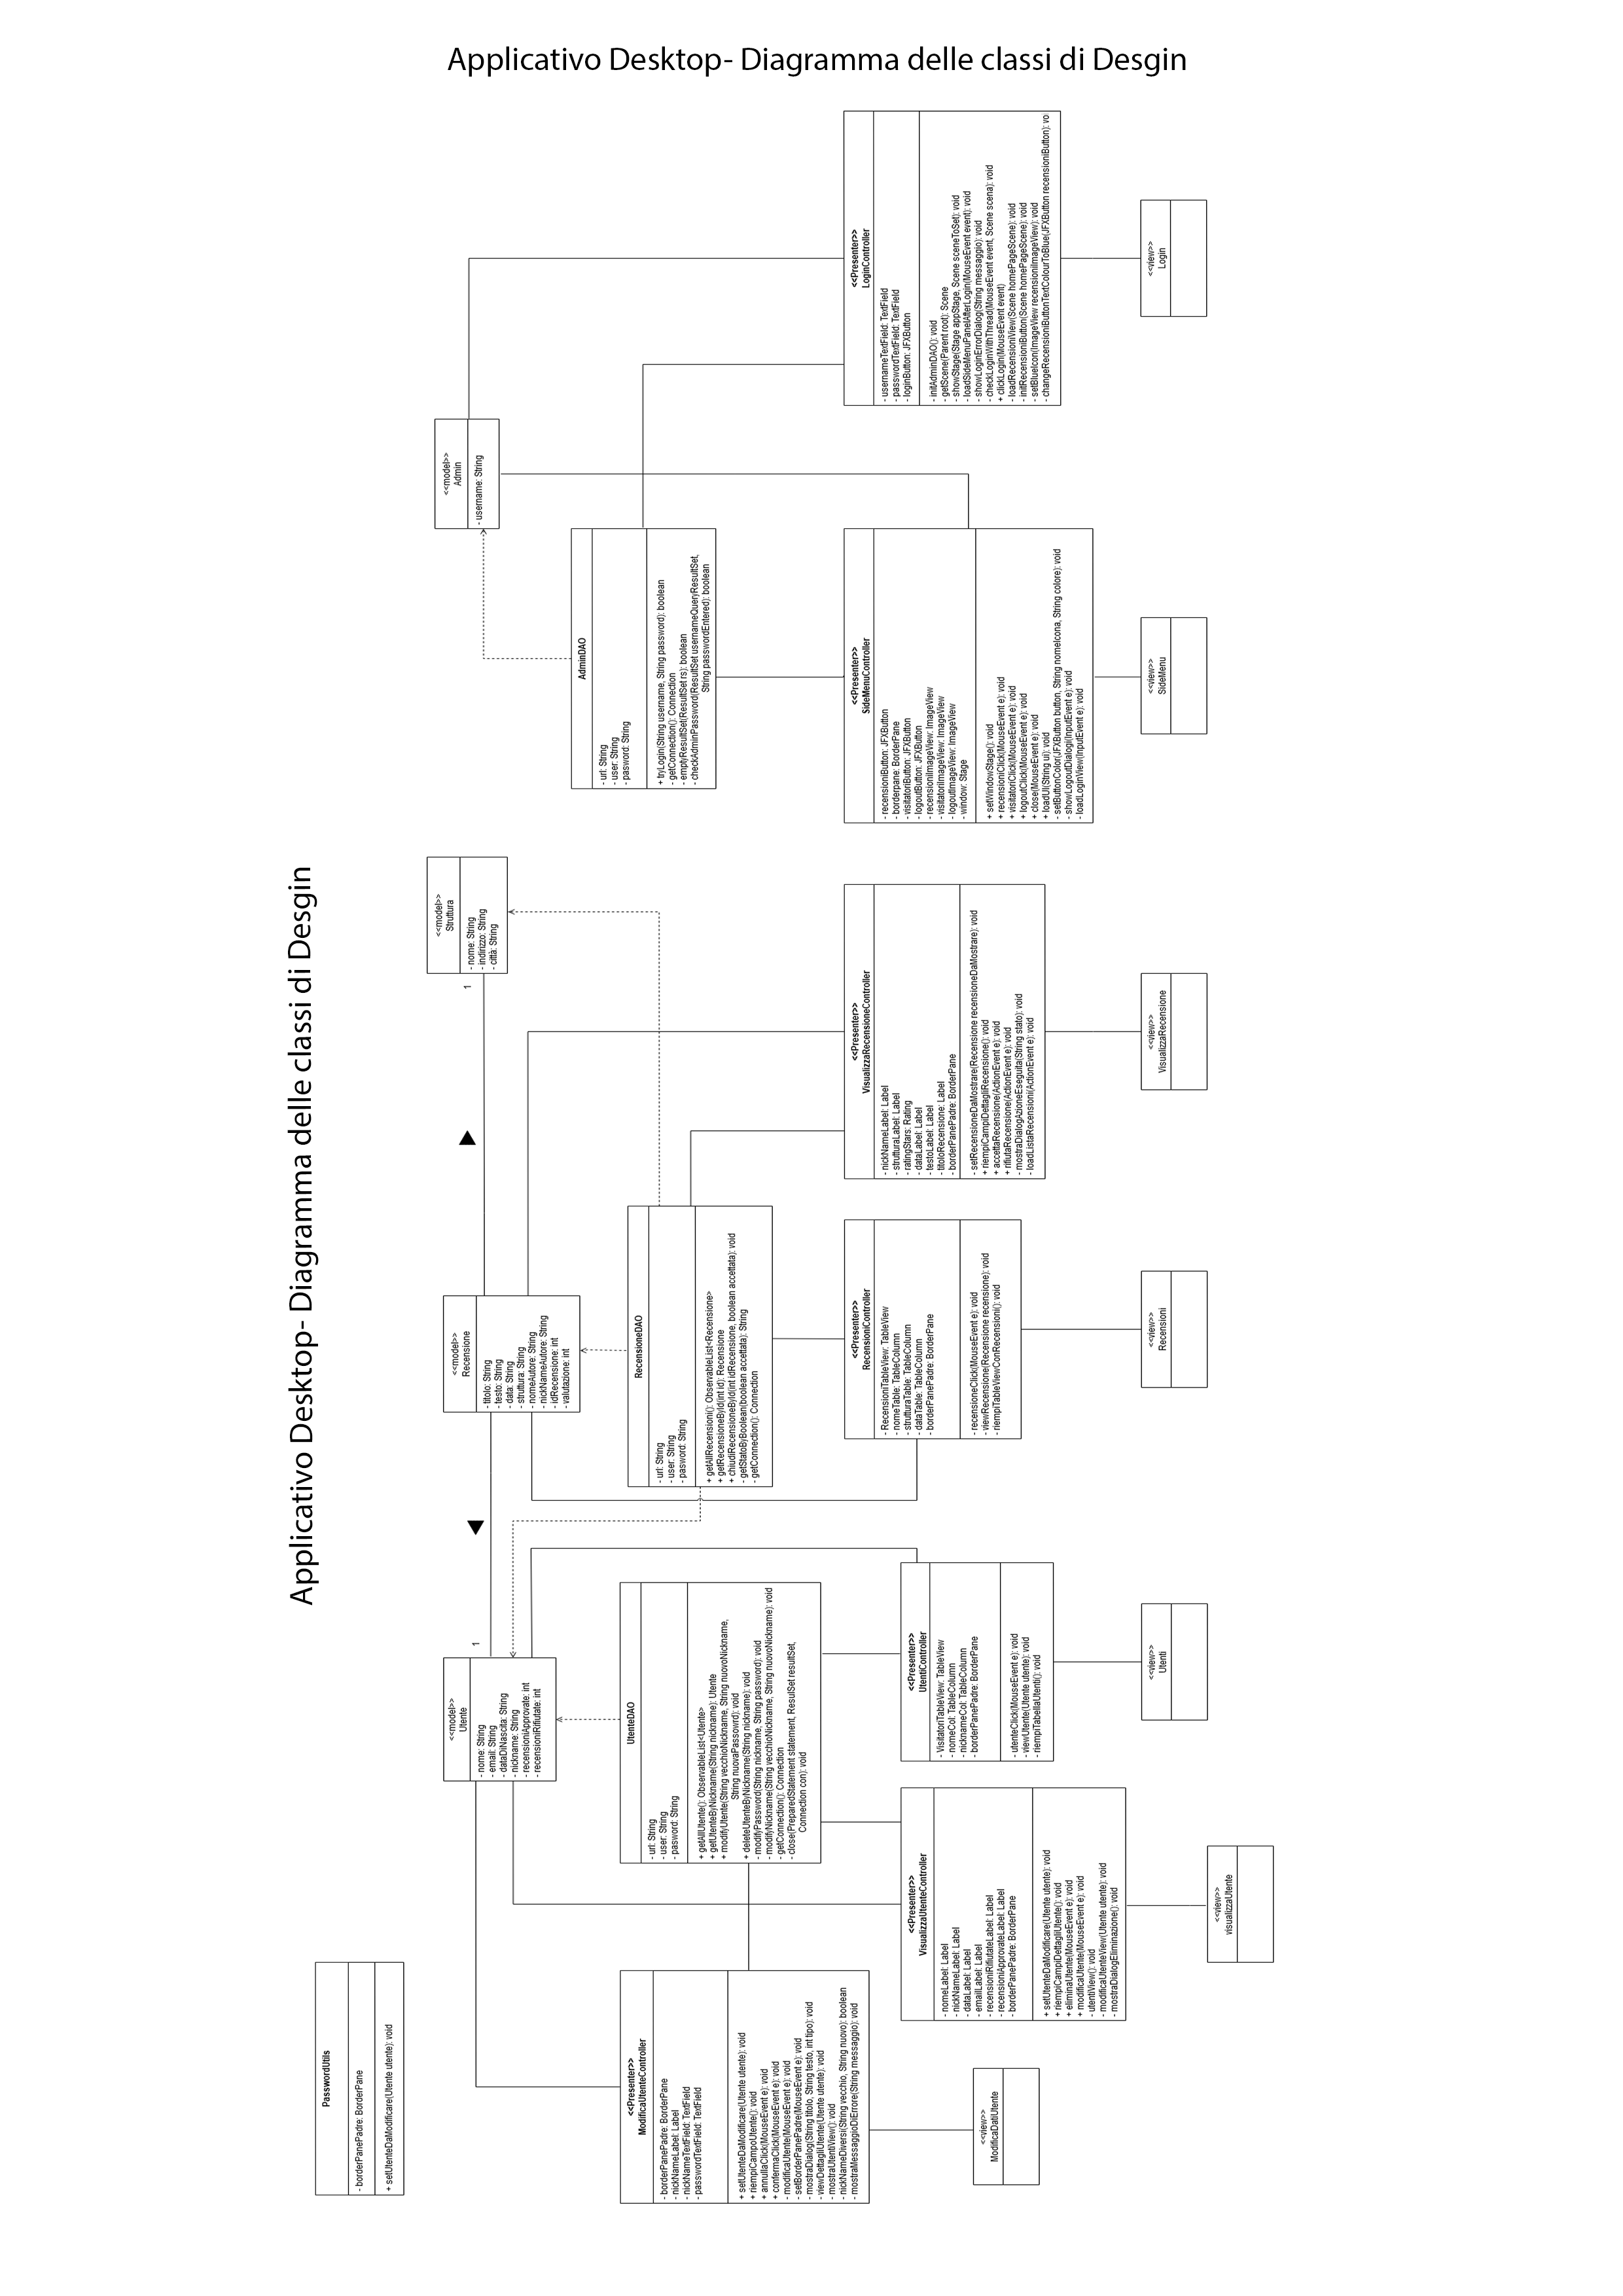
\includegraphics[scale=0.18]{SequenceAnalisi/12.png}
%\end{figure}
\pagebreak

\subsection{Applicativo Mobile}
%\begin{figure}[h!]
%    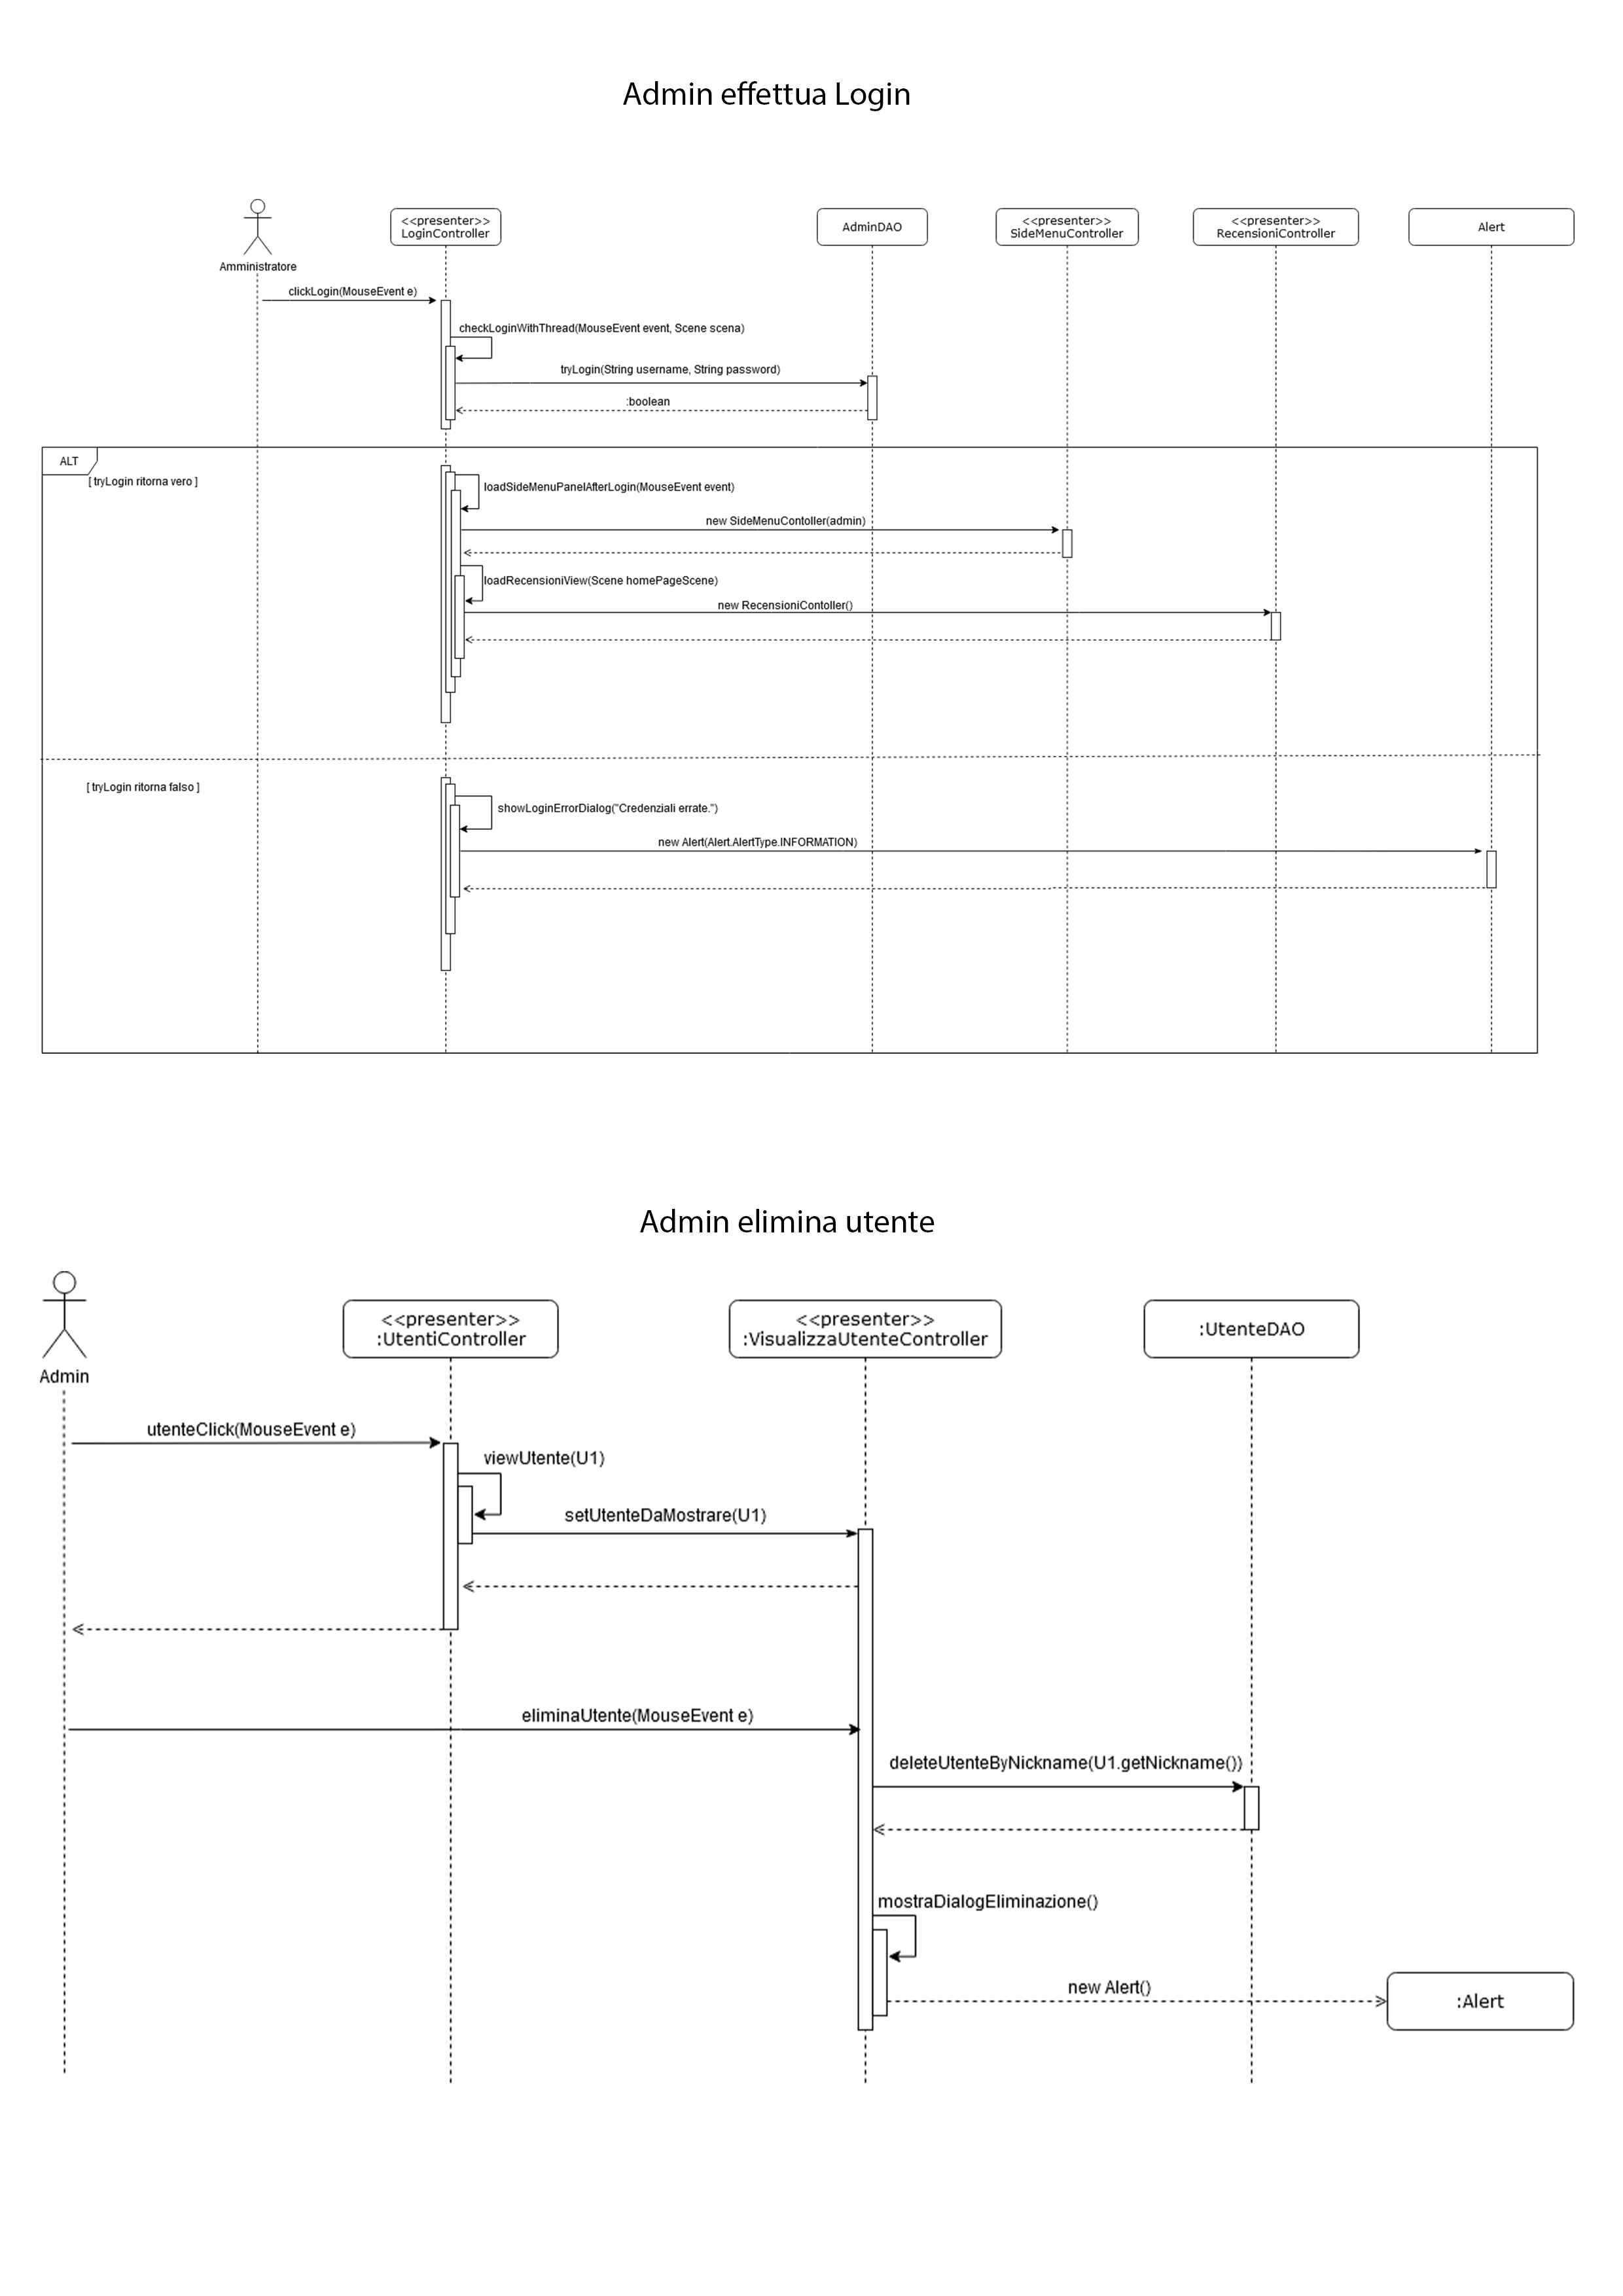
\includegraphics[width=\textwidth]{SequenceAnalisi/13.png}
%\end{figure}
%\pagebreak
%------------------------------------
\section{CRC  Cards}
Di seguitop sono riportate tutte le Class Responsability Collaboration(CRC) del prodotto.

\subsection{Entità}
    
%Intestazione tabella%
\setcounter{table}{0}
\begin{table}[H]
    \centering
    %\caption{AdminDAO} 
    \begin{tabular}{||   l  ||  c   ||}
        \rowcolor{Gray}
        \hline
        Nome Classe & Recensione\\
        \hline
        Superclasse  &  - \\
        \hline
        Sottoclassi & - \\
        \hline
        \hline
         Responsabilità & Collaboratore \\
         \hline
          Rappresentare l'entità Recensione & Utente, Struttura \\
         \hline
    \end{tabular}
    %Continua alla pagina seguente
\end{table}

    
       

    
%Intestazione tabella%
\setcounter{table}{0}
\begin{table}[H]
    \centering
    %\caption{AdminDAO} 
    \begin{tabular}{||   l  ||  c   ||}
        \hline
        Nome Classe & Struttura\\
        \hline
        Superclassi  &  - \\
        \hline
        Sottoclassi & - \\
        \hline
        \hline
         Responsabilità & Collaboratore \\
         \hline
          Rappresentare l'entità Struttura & - \\
         \hline
    \end{tabular}
    %Continua alla pagina seguente
\end{table}

    
       
 
    
%Intestazione tabella%
\setcounter{table}{0}
\begin{table}[H]
    \centering
    %\caption{AdminDAO} 
    \begin{tabular}{||   l  ||  c   ||}
        \hline
        Nome Classe & RecensioneDAO\\
        \hline
        Superclassi  &  - \\
        \hline
        Sottoclassi & - \\
        \hline
         Responsabilità & Collaboratore \\
         \hline
          Effettuare le operazioni CRUD per l'entità Recensione & - \\
         \hline
    \end{tabular}
    %Continua alla pagina seguente
\end{table}

    
%Intestazione tabella%
\setcounter{table}{0}
\begin{table}[H]
    \centering
    %\caption{AdminDAO} 
    \begin{tabular}{||   l  ||  c   ||}
        \hline
        Nome Classe & AdminDAO\\
        \hline
        Superclassi  &  - \\
        \hline
        Sottoclassi & - \\
        \hline
         Responsabilità & Collaboratore \\
         \hline
          Effettuare le operazioni CRUD per l'entità Admin & - \\
         \hline
    \end{tabular}
    %Continua alla pagina seguente
\end{table}

    
       

\subsection{Applicativo Desktop}
    
%Intestazione tabella%
\setcounter{table}{0}
\begin{table}[H]
    \centering
    \begin{tabular}{||   l  ||  c   ||}
        \rowcolor{Gray}
        \hline
        Nome Classe & AdminDAO\\
        \hline
        Superclasse  &  - \\
        \hline
        Sottoclassi & - \\
        \hline
        \hline
         Responsabilità & Collaboratore \\
         \hline
          Effettuare le operazioni CRUD per l'entità Admin & - \\
         \hline
    \end{tabular}
    
    %Continua alla pagina seguente
\end{table}

    
       

    
%Intestazione tabella%
\setcounter{table}{0}
\begin{table}[H]
    \centering
    %\caption{AdminDAO}
    \begin{tabularx}{\textwidth}{||   X  ||  c   ||}
        \rowcolor{Gray}
        \hline
        \textbf{Nome Classe} & UtenteDAO \\
        \hline
        \textbf{Superclasse}  &  - \\
        \hline
        \textbf{Sottoclassi} & - \\
        \hline
        \hline
         \textbf{Responsabilità} & \textbf{Collaboratore} \\
         \hline
          Effettuare le operazioni \gls{CRUD} per l'entità Utente tramite richiesta GET HTTP al web service & - \\
         \hline
    \end{tabularx}
    %Continua alla pagina seguente
\end{table}

    
%Intestazione tabella%
\setcounter{table}{0}
\begin{table}[H]
    \centering
    %\caption{AdminDAO} 
    \begin{tabular}{||   l  ||  c   ||}
        \rowcolor{Gray}
        \hline
        Nome Classe & RecensioneDAO\\
        \hline
        Superclasse  &  - \\
        \hline
        Sottoclassi & - \\
        \hline
        \hline
         Responsabilità & Collaboratore \\
         \hline
          Effettuare le operazioni CRUD per l'entità Recensione & - \\
         \hline
    \end{tabular}
    %Continua alla pagina seguente
\end{table}

    
       

    
%Intestazione tabella%
\setcounter{table}{0}
\begin{table}[H]
    \centering
    %\caption{AdminDAO} 
    \begin{tabular}{||   l  ||  c   ||}
        \rowcolor{Gray}
        \hline
        \textbf{Nome Classe} & LoginPresenter\\
        \hline
        \textbf{Superclasse}  &  - \\
        \hline
        \textbf{Sottoclassi} & - \\
        \hline
        \hline
         \textbf{Responsabilità} & \textbf{Collaboratore} \\
         \hline
          Gestire l'interazione per il login & AdminDAO, Admin \\
         \hline
    \end{tabular}
    %Continua alla pagina seguente
\end{table}


       

    
%Intestazione tabella%
\setcounter{table}{0}
\begin{table}[H]
    \centering
    %\caption{AdminDAO} 
    \begin{tabular}{||   l  ||  c   ||}
        \hline
        \rowcolor{Gray}
        \textbf{Nome Classe} & SideMenuPresenter\\
        \hline
        \textbf{Superclasse}  &  - \\
        \hline
        \textbf{Sottoclassi} & - \\
        \hline
        \hline
         \textbf{Responsabilità} & \textbf{Collaboratore} \\
         \hline
          Gestire l'interazione con la SideBar & Admin \\
         \hline
    \end{tabular}
    %Continua alla pagina seguente
\end{table}

    
       

    
%Intestazione tabella%
\setcounter{table}{0}
\begin{table}[H]
    \centering
    %\caption{AdminDAO} 
    \begin{tabularx}{\textwidth}{||  X  ||  c   ||}
        \rowcolor{Gray}
        \rowcolor{Gray}
        \hline
        \textbf{Nome Classe} & ModificaUtentePresenter\\
        \hline
        \textbf{Superclasse}  &  - \\
        \hline
        \textbf{Sottoclassi} & - \\
        \hline
        \hline
         \textbf{Responsabilità} & \textbf{Collaboratore} \\
         \hline
          Gestire l'interazione per la modifica\newline dei dati di accesso di un utente & Utente, UtenteDAO \\
         \hline
    \end{tabularx}
    %Continua alla pagina seguente
\end{table}

    
       

    
%Intestazione tabella%
\setcounter{table}{0}
\begin{table}[H]
    \centering
    %\caption{AdminDAO} 
    \begin{tabular}{||   l  ||  c   ||}
        \rowcolor{Gray}
        \hline
        \textbf{Nome Classe} & RecensioniPresenter\\
        \hline
        \textbf{Superclasse}  &  - \\
        \hline
        \textbf{Sottoclassi} & - \\
        \hline
        \hline
         \textbf{Responsabilità} & \textbf{Collaboratore} \\
         \hline
          Riempire la tabella con le recensioni in attesa di approvazione & RecensioneDAO \\
         \hline
    \end{tabular}
    %Continua alla pagina seguente
\end{table}

    
       

    
%Intestazione tabella%
\setcounter{table}{0}
\begin{table}[H]
    \centering
    %\caption{AdminDAO} 
    \begin{tabular}{||   l  ||  c   ||}
        \hline
        \rowcolor{Gray}
        \textbf{Nome Classe} & UtentiPresenter\\
        \hline
        \textbf{Superclasse}  &  - \\
        \hline
        \textbf{Sottoclassi} & - \\
        \hline
        \hline
         \textbf{Responsabilità} & \textbf{Collaboratore} \\
         \hline
         Riempire la tabella con gli utenti registrati alla piattaforma & UtenteDAO \\
         \hline
    \end{tabular}
    %Continua alla pagina seguente
\end{table}

    
       

    
%Intestazione tabella%
\setcounter{table}{0}
\begin{table}[H]
    \centering
    %\caption{AdminDAO} 
    \begin{tabular}{||   l  ||  c   ||}
        \hline
        \rowcolor{Gray}
        \textbf{Nome Classe} & VisualizzaRecensionePresenter\\
        \hline
        \textbf{Superclasse}  &  - \\
        \hline
        \textbf{Sottoclassi} & - \\
        \hline
        \hline
         \textbf{Responsabilità} & \textbf{Collaboratore} \\
         \hline
          Gestire l'interazione per la moderazione\newline di una recensione da parte di un admin & RecensioneDAO, Recensione \\
         \hline
    \end{tabular}
    %Continua alla pagina seguente
\end{table}

    
       

    
%Intestazione tabella%
\setcounter{table}{0}
\begin{table}[H]
    \centering
    %\caption{AdminDAO} 
    \begin{tabularx}{\textwidth}{||   X  ||  c   ||}
        \hline
        \rowcolor{Gray}
        \textbf{Nome Classe} & VisualizzaUtentePresenter\\
        \hline
        \textbf{Superclasse}  &  - \\
        \hline
        \textbf{Sottoclassi} & - \\
        \hline
        \hline
         \textbf{Responsabilità} & \textbf{Collaboratore} \\
         \hline
          Mostrare i dati completi di un utente & UtenteDAO, Utente \\
         \hline
          Permette l'eliminazione dell'utente mostrato& UtenteDAO, Utente \\
         \hline
    \end{tabularx}
    %Continua alla pagina seguente
\end{table}

    
       

    
%Intestazione tabella%
\setcounter{table}{0}
\begin{table}[H]
    \centering
    %\caption{AdminDAO} 
    \begin{tabularx}{\textwidth}{||   X  ||  c   ||}
        \rowcolor{Gray}
        \hline
        \textbf{Nome Classe} & PasswordUtils\\
        \hline
        \textbf{Superclasse}  &  - \\
        \hline
        \textbf{Sottoclassi} & - \\
        \hline
        \hline
         \textbf{Responsabilità} & \textbf{Collaboratore} \\
         \hline
          Fornire funzionalità per il sistema di cifratura\newline delle password tramite sale (?)  & - \\
         \hline
    \end{tabularx}
    %Continua alla pagina seguente
\end{table}

    
       

    
%Intestazione tabella%
\setcounter{table}{0}
\begin{table}[H]
    \centering
    %\caption{AdminDAO} 
    \begin{tabular}{||   l  ||  c   ||}
        \rowcolor{Gray}
        \hline
        Nome Classe & AdminDAO\\
        \hline
        Superclasse  &  - \\
        \hline
        Sottoclassi & - \\
        \hline
         Responsabilità & Collaboratore \\
         \hline
          Effettuare le operazioni CRUD per l'entità Admin & - \\
         \hline
    \end{tabular}
    %Continua alla pagina seguente
\end{table}

    
       

    \pagebreak
\subsection{Applicativo Mobile}
    
%Intestazione tabella%
\setcounter{table}{0}
\begin{table}[H]
    \centering
    %\caption{AdminDAO}
    \begin{tabularx}{\textwidth}{||   X  ||  c   ||}
        \rowcolor{Gray}
        \hline
        \textbf{Nome Classe} & UtenteDAO \\
        \hline
        \textbf{Superclasse}  &  - \\
        \hline
        \textbf{Sottoclassi} & - \\
        \hline
        \hline
         \textbf{Responsabilità} & \textbf{Collaboratore} \\
         \hline
          Effettuare le operazioni \gls{CRUD} per l'entità Utente tramite richiesta GET HTTP al web service & - \\
         \hline
    \end{tabularx}
    %Continua alla pagina seguente
\end{table}

    
%Intestazione tabella%
\setcounter{table}{0}
\begin{table}[H]
    \centering
    %\caption{AdminDAO} 
    \begin{tabular}{||   l  ||  c   ||}
        \rowcolor{Gray}
        \hline
        Nome Classe & RecensioneDAO\\
        \hline
        Superclasse  &  - \\
        \hline
        Sottoclassi & - \\
        \hline
        \hline
         Responsabilità & Collaboratore \\
         \hline
          Effettuare le operazioni CRUD per l'entità Recensione & - \\
         \hline
    \end{tabular}
    %Continua alla pagina seguente
\end{table}

    
       

    
%Intestazione tabella%
\setcounter{table}{0}
\begin{table}[H]
    \centering
    %\caption{AdminDAO} 
    \begin{tabular}{||   l  ||  c   ||}
        \hline
        Nome Classe & RecensioneDAO\\
        \hline
        Superclassi  &  - \\
        \hline
        Sottoclassi & - \\
        \hline
         Responsabilità & Collaboratore \\
         \hline
          Effettuare le operazioni CRUD per l'entità Recensione & - \\
         \hline
    \end{tabular}
    %Continua alla pagina seguente
\end{table}

    
%Intestazione tabella%
\setcounter{table}{0}
\begin{table}[H]
    \centering
    %\caption{AdminDAO} 
    \begin{tabular}{||   l  ||  c   ||}
        \hline
        Nome Classe & RecensioneDAO\\
        \hline
        Superclassi  &  - \\
        \hline
        Sottoclassi & - \\
        \hline
         Responsabilità & Collaboratore \\
         \hline
          Effettuare le operazioni CRUD per l'entità Recensione & - \\
         \hline
    \end{tabular}
    %Continua alla pagina seguente
\end{table}

    
%Intestazione tabella%
\setcounter{table}{0}
\begin{table}[H]
    \centering
    %\caption{AdminDAO} 
    \begin{tabularx}{\textwidth}{||   X  ||  c   ||}
        \hline
        \rowcolor{Gray}
        \textbf{Nome Classe} & DettagliStrutturaFragment\\
        \hline
        Superclassi  &  - \\
        \hline
        \textbf{Sottoclassi} & - \\
        \hline
        \hline
         \textbf{Responsabilità} & \textbf{Collaboratore} \\
         \hline
          Permette la visualizzazione dei dati di una struttura & Struttura, RecensioneDAO \\
         \hline
    \end{tabularx}
    %Continua alla pagina seguente
\end{table}

    
%Intestazione tabella%
\setcounter{table}{0}
\begin{table}[H]
    \centering
    %\caption{AdminDAO} 
    \begin{tabular}{||   l  ||  c   ||}
        \hline
        \rowcolor{Gray}
        \textbf{Nome Classe} & LoginFragment\\
        \hline
        Superclassi  &  - \\
        \hline
        \textbf{Sottoclassi} & - \\
        \hline
         \textbf{Responsabilità} & \textbf{Collaboratore} \\
         \hline
           Gestisce l'accesso, tramite credenziali, di un utente & UtenteDAO \\
         \hline
    \end{tabular}
    %Continua alla pagina seguente
\end{table}

    
%Intestazione tabella%
\setcounter{table}{0}
\begin{table}[H]
    \centering
    %\caption{AdminDAO} 
    \begin{tabularx}{\textwidth}{||   X  ||  c   ||}
        \hline
        \rowcolor{Gray}
        \textbf{Nome Classe} & NessunaStrutturaTrovata\\
        \hline
        Superclassi  &  - \\
        \hline
        \textbf{Sottoclassi} & - \\
        \hline
        \hline
         \textbf{Responsabilità} & \textbf{Collaboratore} \\
         \hline
           Mostra una schermata apposita nel caso in cui una ricerca
           non abbia nessun risultato da visualizzare & - \\
         \hline
    \end{tabularx}
    %Continua alla pagina seguente
\end{table}

    
%Intestazione tabella%
\setcounter{table}{0}
\begin{table}[H]
    \centering
    %\caption{AdminDAO} 
    \begin{tabular}{||   l  ||  c   ||}
        \hline
        Nome Classe & RecensioneDAO\\
        \hline
        Superclassi  &  - \\
        \hline
        Sottoclassi & - \\
        \hline
         Responsabilità & Collaboratore \\
         \hline
          Effettuare le operazioni CRUD per l'entità Recensione & - \\
         \hline
    \end{tabular}
    %Continua alla pagina seguente
\end{table}

    
%Intestazione tabella%
\setcounter{table}{0}
\begin{table}[H]
    \centering
    %\caption{AdminDAO} 
    \begin{tabularx}{\textwidth}{||   X  ||  c   ||}
        \hline
        \rowcolor{Gray}
        \textbf{Nome Classe} & VisualizzaRecensioneFragment\\
        \hline
        Superclassi  &  - \\
        \hline
        \textbf{Sottoclassi} & - \\
        \hline
         \textbf{Responsabilità} & \textbf{Collaboratore} \\
         \hline
          Permette la visualizzazione (con testo integrale) di una Recensione  & Recensione \\
         \hline
    \end{tabularx}
    %Continua alla pagina seguente
\end{table}

    
%Intestazione tabella%
\setcounter{table}{0}
\begin{table}[H]
    \centering
    %\caption{AdminDAO} 
    \begin{tabularx}{\textwidth}{||   X  ||  c   ||}
        \hline
        \rowcolor{Gray}
        \textbf{Nome Classe} & VisualizzaStrutturaSuSMappa\\
        \hline
        Superclassi  &   \\
        \hline
        \textbf{Sottoclassi} & - \\
        \hline
         \textbf{Responsabilità} & \textbf{Collaboratore} \\
         \hline
          Permette di visualizzare su mappa la posizione di una Struttura & Struttura \\
         \hline
    \end{tabularx}
    %Continua alla pagina seguente
\end{table}

%------------------------------------
\section{Diagramma di stato di design}

\section{Diagramma di sequenza di design}